\documentclass[10pt,landscape, a4paper]{article}
\usepackage{multicol}
\usepackage{calc}
\usepackage{ifthen}
\usepackage[landscape]{geometry}
\usepackage{amsmath,amsthm,amsfonts,amssymb}
\usepackage{bm}
\usepackage{graphicx}
\graphicspath{ {./images/st2334/} }


\pdfinfo{
  /Title (ST2334 Cheatsheet)
  /Creator (Tony Kwong)
  /Producer (pdfTeX 1.40.0)
  /Subject (ST2334 Statistics \& Probability)
  /Keywords (pdflatex, latex,pdftex,tex)}

% This sets page margins to .5 inch if using letter paper, and to 1cm
% if using A4 paper. (This probably isn't strictly necessary.)
% If using another size paper, use default 1cm margins.
\ifthenelse{\lengthtest { \paperwidth = 11in}}
    { \geometry{top=.5in,left=.5in,right=.5in,bottom=.5in} }
    {\ifthenelse{ \lengthtest{ \paperwidth = 297mm}}
        {\geometry{top=1cm,left=1cm,right=1cm,bottom=1cm} }
        {\geometry{top=1cm,left=1cm,right=1cm,bottom=1cm} }
    }

% Turn off header and footer
\pagestyle{empty}

% Redefine section commands to use less space
\makeatletter
\renewcommand{\section}{\@startsection{section}{1}{0mm}%
                                {-1ex plus -.5ex minus -.2ex}%
                                {0.5ex plus .2ex}%x
                                {\normalfont\large\bfseries}}
\renewcommand{\subsection}{\@startsection{subsection}{2}{0mm}%
                                {-1explus -.5ex minus -.2ex}%
                                {0.5ex plus .2ex}%
                                {\normalfont\normalsize\bfseries}}
\renewcommand{\subsubsection}{\@startsection{subsubsection}{3}{0mm}%
                                {-1ex plus -.5ex minus -.2ex}%
                                {1ex plus .2ex}%
                                {\normalfont\small\bfseries}}
\makeatother

% Define BibTeX command
\def\BibTeX{{\rm B\kern-.05em{\sc i\kern-.025em b}\kern-.08em
    T\kern-.1667em\lower.7ex\hbox{E}\kern-.125emX}}

% print only section numbers
\setcounter{secnumdepth}{1}


\setlength{\parindent}{0pt}
\setlength{\parskip}{0pt plus 0.5ex}

%My Environments
\newtheorem{example}[section]{Example}


% -----------------------------------------------------------------------

\begin{document}
\raggedright
\footnotesize
\begin{multicols}{3}


% multicol parameters
% These lengths are set only within the two main columns
%\setlength{\columnseprule}{0.25pt}
\setlength{\premulticols}{1pt}
\setlength{\postmulticols}{1pt}
\setlength{\multicolsep}{1pt}
\setlength{\columnsep}{2pt}

\begin{flushleft}
\large{
    \underline{ST2334 Cheat Sheet}
    }
\end{flushleft}

% ------------------------------ACTUAL CONTENT-----------------------------------
\section{Probability}
\subsection{De Morgan's Law}
\[ (A \cup B)^\prime = A^\prime \cap B^\prime \] \\
\[ (A \cap B)^\prime = A^\prime \cup B^\prime \] \\

\subsection{Permutation \& Combination}
\[ P^{n}_{r} = \frac{n!}{(n-r)!} = n(n-1)(n-2)...(n-(r-1)) \] \\
\[ C^{n}_{r} = \frac{n!}{r!(n-r)!} \] \\

\subsection{Properties}
\[ P(A) = P(A \cap B) + P(A \cap B^\prime) \] \\
\[ P(A \cup B) = P(A) + P(B) - P(A \cap B) \] \\
\[ A \subset B \rightarrow P(A) \leq P(B) \] \\

\subsection{Conditional Probability}
\[ P(B|A) = \frac{P(A \cap B)}{P(A)} \] \\

\subsection{Inverse Probability Formula}
\[ P(A|B) = \frac{P(A)P(B|A)}{P(B)} \] \\

\subsection{Independence}
\[ A \perp B \iff P(A \cap B) = P(A)P(B) \] \\
\[ A \perp B \iff P(B|A) = P(B) \] \\
The knowledge of A doesn't change the probability of B

\subsection{Law of Total Probability}
\[ P(B) = P(A)P(B|A) + P(A^\prime)(P(B|A^\prime) \] \\

\subsection{Bayes' Theorem}
Probability of an event based on knowledge of related conditions
\[ P(A|B) = \frac{P(A)P(B|A)}{P(A)P(B|A) + P(A^\prime)P(B|A^\prime)} = \frac{P(A)P(B|A)}{P(B)} \] \\


\section{Random Variables}
\subsection{Notations}
Random variables: \(X_1\), \(X_2\), \(Y_1\), \(Y_2\), \(Z_1\), \(Z_2\) \\
Observed values: \(x_1\), \(x_2\), \(y_1\), \(y_2\), \(z_1\), \(z_2\) \\
\[ \{X = x\} = \{s \in S : X(s) = x\} \] \\
The set \(\{X = 0\}\) is the set of outcomes in the sample space when \(X(s) = 0\) \\

\subsection{Discrete Random Variables}
The range of \(X\) \(R_X\) is finite or countable \\

\subsubsection{Probability Mass Function (PMF)}
\[
    f(x) = 
        \begin{cases}
            P(X = x), & \text{for } x \in R_X  \\
            0, & \text{for } x \notin R_X  \\
        \end{cases}
\] \\

Properties
\begin{enumerate}
    \item \(f(x_i) \geq 0\) for all \(x_i \in R_X\)
    \item \(f(x) = 0\) for all \(x \notin R_X\)
    \item Sum of individual probability functions is 1
\end{enumerate}

\subsection{Continuous Random Variables}
\(R_X\) is an interval or collection of intervals \\

\subsubsection{Probability Density Function (PDF)}
Properties
\begin{enumerate}
    \item \(f(x_i) \geq 0\) for all \(x_i \in R_X\)
    \item \(f(x) = 0\) for all \(x \notin R_X\)
    \item \( \int_{R_X} f(x) dx = 1 \)
    \item \( P(a \leq X \leq b) = \int^{b}_{a} f(x) dx \)
\end{enumerate}
For any specific value \(x_0\), \(P(x_0) = 0\) \\
Also,
\[ P(a < X < b) = P(a < X \leq b) = P(a \leq X < b) = P(a \leq X \leq b)  \] \\
To check if \(f(x)\) is a PDF, ensure that 1 \& 2 \& 3 are true 

\subsection{Culmulative Distribution Function}
For both discrete \& continuous random variables,
\[ F(x) = P(X \leq x) \] \\

\subsubsection{Discrete}
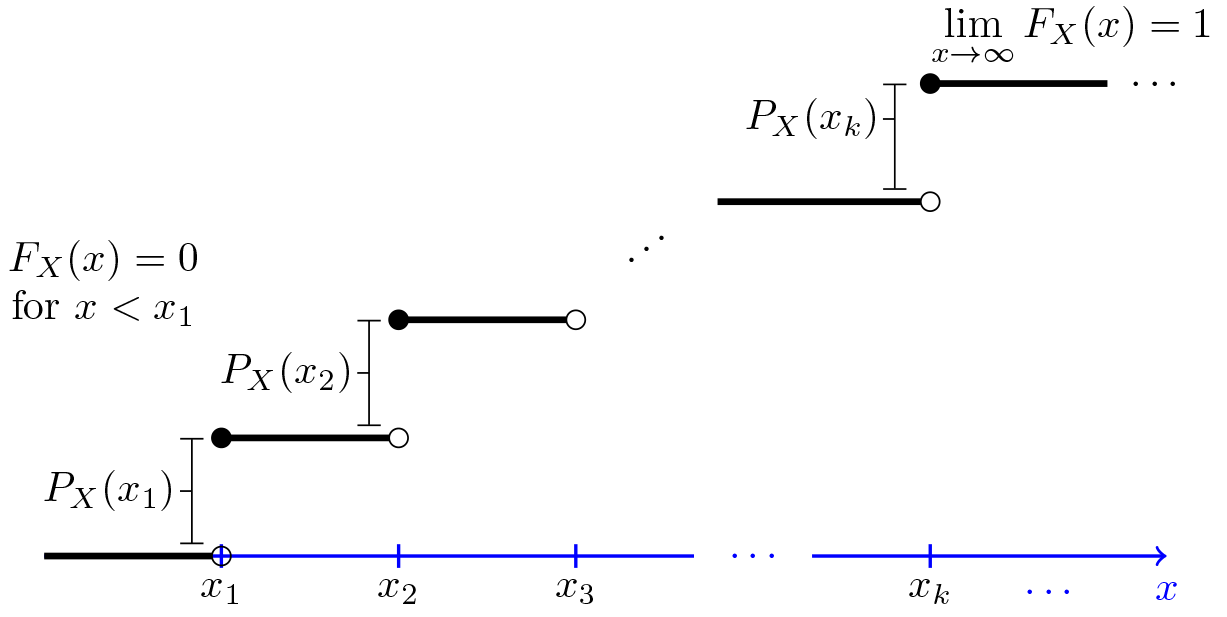
\includegraphics[width=8cm]{cdf-discrete}

\subsubsection{Continuous}
\[ F(x) = \int^{x}_{-\infty} f(t) dt \] \\
\[ f(x) = \frac{dF(x)}{dx} \] \\
\(-\infty\) can be replaced by the "lower limit" since \( f(x) = 0 \), for all \( x \notin R_X \) \\
Integrate PDF to get CDF, and vice versa \\

\subsection{Expectation/Mean}
\[\mu_x = E(X)\]
\subsubsection{Discrete}
\[ E(X) = \sum\limits_{x_i \in R_X} x_i f(x_i) \] \\
Sum of all individual probabilities multipled by the respective values

\subsubsection{Continuous}
\[ E(X) = \int^{\infty}_{-\infty} x f(x) dx \] \\
Similarly, limits can be replaced

\subsubsection{Properties}
\begin{enumerate}
    \item \(E(aX + b) = aE(X) + b\)
    \item \(E(X + Y) = E(X) + E(Y)\)
    \item Discrete: \( E[g(X)] = \sum\limits_{x \in R_X} g(x)f(x) \)
    \item Continuous: \( E[g(X)] = \int_{R_X} g(x)f(x) dx \)
\end{enumerate}

\subsection{Variance}
\[\sigma^{2}_{X} = V(X) = E(X - \mu_x)^2\] \\

\subsubsection{Computational Formula}
\[ V(X) = E(X^2) - E(X)^2 \] \\

\subsubsection{Standard Deviation}
\[ \sigma_x = \sqrt{V(X)} \] \\
In a bell curve (normal distribution), ~68\% of values are within \(\pm1 \sigma\) from the mean 

\end{multicols}
\end{document}
